\qrchapter{https://forgottenpillar.com/rsc/hr-fp-chapter1}{Temelj Naše Vjere}

\egw{\textbf{Gospodin će podariti novu, životnu silu u svoj rad} kada ljudski podanici poslušaju zapovijed da izađu i nagovijeste istinu. \textbf{Onaj koji je objavio da će Njegova istina zauvijek sjajiti, objaviti će tu istinu kroz vjerne glasnike, koji će zatrubiti pouzdan zvuk}. \textbf{Istina će biti kritizirana, prezrena i ismijavana; ali što će se \underline{bolje} provjeravati i testirati, \underline{snažnije će svijetliti}}.}[SpTB02 51.1; 1904][https://egwwritings.org/read?panels=p417.260]

\egwnogap{\textbf{Kao narod moramo \underline{čvrsto stajati na platformi vječne istine} koja je izdržala test i probu. Moramo se \underline{držati sigurnih stupova naše vjere}. \underline{Principi istine}, koje nam je Bog objavio, su \underline{naš jedini istiniti temelj}. Oni su nas učinili onim što jesmo. Protek vremena nije umanjilo njihovu vrijednost. \underline{Stalni je napor neprijatelja da ukloni ove istine sa njihovog mjesta}, i umjesto njih postavi \underline{lažne teorije}. On će \underline{unijeti} sve što je u mogućnosti kako bi ostvario svoje varljive nakane. No, Gospodin će podići ljude oštroumnog rasuđivanja, koji će ovim istinama dati njihovo pravo mjesto u Božjem planu.}}[SpTB02 51.2; 1904][https://egwwritings.org/read?panels=p417.261]

\egwnogap{\textbf{Bila sam upućena od strane Nebeskog glasnika da su neka rasuđivanja u knjizi ‘Živi Hram’ netočna i da će \underline{ta razmišljanja odvesti u zabludu} umove onih koji nisu temeljito utemeljeni na \underline{temeljnim principima} sadašnje istine. Ona uvode ono što je ništa više nego obična nagađanja \underline{vezano za ličnost Boga i gdje je Njegova prisutnost}}. Nitko na ovoj zemlji nema pravo nagađati o tom pitanju. \textbf{Što se više o tim izmišljenim teorijama raspravlja, manje ljudi će znati o Bogu i istinama koje posvećuje dušu}.}[SpTB02 51.3; 1904][https://egwwritings.org/read?panels=p417.262]


\egwnogap{Jedan za drugim dolaze k meni, tražeći me \textbf{da objasnim stajališta u knjizi ‘Živi Hram’}. Odgovaram: ‘\textbf{Oni su neobjašnjivi}’. \textbf{Izraženi sentimenti ne daju istinsko znanje o Bogu}. Kroz cijelu knjigu su odlomci Svetog Pisma. Pismo je korišteno na takav način da se zabludu prikaže kao istinu. \textbf{Pogrešne teorije su prikazane na tako ugodan način da, ukoliko se ne bude oprezan, mnogi će biti zavedeni}.}[SpTB02 52.1; 1904][https://egwwritings.org/read?panels=p417.265]

\egwnogap{\textbf{Mi ne trebamo misticizam koji je u toj knjizi}. Oni koji zagovaraju ove zablude uskoro će se naći u poziciji gdje će neprijatelj moći razgovarati s njima i odvesti ih od Boga. Predstavljeno mi je da je pisac ove knjige na pogrešnoj stazi. \textbf{Izgubio je iz vida posebite istine za \underline{ovo vrijeme}}. On ne zna gdje ga njegovi koraci vode. \textbf{\underline{Staza istine leži blizu staze zablude}, i obje staze mogu izgledati jednake u umovima koji nisu vođeni Duhom Svetim, i koji, stoga, nisu sposobni brzo razlučiti razliku između istine i zablude}.}[SpTB02 52.2; 1904][https://egwwritings.org/read?panels=p417.266]

\egwnogap{\textbf{U vremenu kada se izdala knjiga ‘Živi Hram’, u noćnoj viziji, \underline{predstavljeni su mi prikazi koji su ukazivali na približavanje neke opasnosti}, te da se za nju moram pripremiti \underline{pisanjem stvari} koje mi je Bog objavio \underline{vezano za temeljne principe naše vjere}}.}[SpTB02 52.3; 1904][https://egwwritings.org/read?panels=p417.267]

\egwnogap{Poslana mi je kopija ‘Živog Hrama’, ali je ostala u mojoj knjižnici, nepročitana. Od svjetlosti koju mi je dao Gospodin, \textbf{znala sam da neki od sentimenata koji se zagovaraju u knjizi nisu nosili Božje odobrenje}, \textbf{i da su oni \underline{zamka koju je neprijatelj pripremio za posljednje dane}}. Mislila sam da će to sigurno biti primjećeno i da neće biti nužno reći nešto o tome.}[SpTB02 52.4; 1904][https://egwwritings.org/read?panels=p417.268]

\egwnogap{U kontraverzi koja je nastala među našom braćom u vezi s učenjima ove knjige, \textbf{oni koji podupiru njezinu široku cirkulaciju izjavili su: ‘Ona sadrži upravo one sentimente koje Sestra White podučava’}. Ova tvrdnja pogodila je moje srce. Osjećala sam se slomljenom; jer \textbf{sam znala da takva prikazivanja stvari \underline{nisu istinita}}.}[SpTB02 53.1; 1904][https://egwwritings.org/read?panels=p417.270]

\egwnogap{Konačno, moj sin mi je rekao: ‘Majko, treba bi pročitati barem neke dijelove knjige kako bi vidjela jesu li u skladu s svjetlom koje ti je Bog dao’. Sjeo je pored mene i zajedno \textbf{smo pročitali predgovor i većinu prvog poglavlja, kao i odlomke u drugim poglavljima}. Dok smo čitali, prepoznala sam upravo one sentimente protiv kojih sam bila pozvana upozoravati \textbf{tijekom \underline{ranih dana} mojeg javnog djelovanja}. Kada sam prvi put napustila državu Maine, trebala sam proći Vermont i Massachusetts, kako bi svjedočila protiv tih sentimenata. \textbf{‘Živi Hram’ sadrži alfu tih teorija. Znala sam da će \underline{omega ubrzo uslijediti}; i drhtala sam za naš narod}. \textbf{Znala sam da moram upozoriti našu braću i sestre da ne ulaze u kontroverzu \underline{oko prisutnosti i ličnosti Boga}}. \textbf{Sentimenti u knjizi ‘Živi Hram’ \underline{vezani za tu točku su netočni}}. Sveto Pismo koje se koristilo za potkrijepljenje te doktrine, je pogrešno primijenjeno.}[SpTB02 53.2; 1904][https://egwwritings.org/read?panels=p417.271]

\egwnogap{\textbf{Primorana sam govoriti i odbiti tvrdnje da se učenja ‘Živog Hrama’ mogu poduprijeti tvrdnjama iz mojih spisa}. \textbf{U toj knjizi mogu postojati izrazi i sentimenti koji su u skladu s mojim spisima}. \textbf{U mojim spisima mogu biti mnoge tvrdnje koje, uzete iz njihovog konteksta i tumačene prema umu pisca ‘Živog Hrama’, čini se da su u skladu s učenjima ove knjige}. To može dati prividnu potporu tvrdnji da su sentimenti u ‘Živom Hramu’ u skladu s mojim spisima. \textbf{Ali, Bože sačuvaj da taj sentiment prevlada}.}[SpTB02 53.3; 1904][https://egwwritings.org/read?panels=p417.272]

\egwnogap{\textbf{Malo tko može razabrati rezultat gajenja zabluda koji neki zagovaraju u ovom trenutku}. \textbf{Ali Gospod je podigao zavjesu i \underline{pokazao mi rezultat koji bi uslijedio}}. \textbf{Spiritualističke teorije o \underline{ličnosti Boga}, praćene njihovim logičnim zaključkom, oduzimaju cjelokupno kršćansko razumijevanje}. \textbf{One nimalo ne vrednuju svjetlo, zbog kojeg je Krist s neba došao da bi ga dao Ivanu, a dao Njegovom narodu. One poučavaju da događaji pred nama nisu dovoljno važni da im se posveti posebna pažnja. One uništavaju učinkovitost istine nebeskog porijekla i \underline{liše Božji narod njihovog prošlog iskustva}, zauzvrat dajući im lažne znanosti}.}[SpTB02 54.1; 1904][https://egwwritings.org/read?panels=p417.275]

\egwnogap{\textbf{U noćnoj viziji} bilo mi je jasno pokazano da se \textbf{na te sentimente} od nekih gleda kao na \textbf{velike istine} \textbf{koje se trebaju \underline{uvesti}} i učiniti ih važnima u današnje vrijeme. \textbf{Pokazano mi je \underline{platforma}, poduprta \underline{čvrstim stupovima},—istinama Riječi Božje}. \textbf{Netko visoke odgovornosti u zdravstvenom radu usmjeravao je tog čovjeka da rasklima stupove koji podržavaju ovu platformu}. Tada sam čula glas koji govori: ‘Gdje su stražari koji bi trebali stajati na zidovima Siona? Da li su zaspali? \textbf{\underline{Ovaj temelj je izgrađen od strane Najvećeg Radnika}, i \underline{održati će se} na oluji i buri. Hoće li mu se dopustiti da ovaj čovjek \underline{predstavi doktrine} koje \underline{opovrgavaju prošlo iskustvo} Božjeg naroda? Došlo je vrijeme za odlučnu akciju}.’}[SpTB02 54.2; 1904][https://egwwritings.org/read?panels=p417.276]

\egwnogap{\textbf{Neprijatelj duša tražio je da \underline{uvede} pretpostavku da će nastati \underline{velika reformacija} među Adventistima Sedmog Dana, i da će se \underline{ta reforma} \underline{sačinjavati od odstupanja od doktrina koje stoje kao stupovi naše vjere,} i da će se pokrenuti proces reorganizacije}. \textbf{Kada bi takva reformacija nastupila, \underline{kakav bi bio rezultat}?} \textbf{\underline{Principi istine} koje Bog u svojoj mudrosti dao crkvi ostatka \underline{bili bi odbačeni}}. \textbf{Naša religija bi se promijenila}. \textbf{\underline{Fundamentalni principi} koji su održavali posao posljednjih pedeset godina \underline{bili bi proglašeni greškom}}. \textbf{Nova organizacija bi se osnovala}. \textbf{Knjige novog reda bi se napisale}. \textbf{Uveo bi se sistem intelektualne filozofije}. Osnivači ovog pokreta išli bi u gradove i napravili nevjerojatan posao. Naravno, subota bi se olako smatrala, \textbf{kao i Boga koji ju je stvorio}. Ničemu ne bi bilo dopušteno stajati na putu novom pokretu. \textbf{Vođe bi poučavali da je vrlina bolja od poroka, ali kako je \underline{Bog uklonjen}, oni će staviti svoju ovisnost na ljudske snage koje su, bez Boga, bezvrijedne}. \textbf{Njihov temelj će biti izgrađen na pijesku, a oluja i bura će odnijeti strukturu}.}[SpTB02 54.3; 1904][https://egwwritings.org/read?panels=p417.277]

\egwnogap{Tko ima ovlasti započeti takav pokret? \textbf{Imamo naše Biblije}. \textbf{Imamo svoje iskustvo koje potvrđeno čudesnim radom Duha Svetoga}. \textbf{Imamo istinu koja ne prihvaća kompromise}. \textbf{\underline{Ne bismo li trebali odbacili sve što nije u skladu s tom istinom}}?}[SpTB02 55.1; 1904][https://egwwritings.org/read?panels=p417.280]

\egwnogap{Oklijevala sam i zadržavala sam se oko slanja onoga što mi je Duh Gospodnji potaknuo da napišem. \textbf{Nisam željela biti prisiljena predstaviti zavaravajući utjecaj tih zabluda. Ali u Božjoj providnosti, zablude koje ulazile moraju biti suočene}.}[SpTB02 55.2; 1904][https://egwwritings.org/read?panels=p417.281]

\egwnogap{Prije nego što sam poslala \textbf{svjedočanstva o \underline{naporima neprijatelja da potkopa temelje naše vjere} kroz širenje \underline{zavodljivih teorija}}, pročitala sam o incidentu o brodu koji se suočio sa ledenjakom u magli. Već nekoliko noći malo spavam. Osjećala sam se kao pognuti snopovi ispod srpa. Jedne noći pokazala mi je jasna scena predamnom. Brod je bio na vodi, u teškoj magli. Odjednom je osmatrač uzviknuo, ‘Ledenjak ispred nas!’ Visoko iznad broda, podizao se ogroman ledeni brijeg. Autoritativan glas je uzviknuo: ‘Suoči se!’ Nije bilo trenutka za oklijevanje. Bilo je vrijeme za trenutnu akciju. Inženjer je dao punu paru, a čovjek na kormilu okreće brod ravno u ledeni brijeg. Sa velikim udarcem je razlomio led. Bilo je strahovito šokantno, a ledeni brijeg razlomio se u mnoge dijelove, sa bukom poput grmljavine na palubu. Putnici su silno potreseni od sile sudara, ali nijedan život nije izgubljen. Brod je oštećen, ali ne da se ne može popraviti. Odbio se od udara, dršćući od repa do krme, poput živog bića. Zatim je nastavio dalje svojim putem.}[SpTB02 55.3; 1904][https://egwwritings.org/read?panels=p417.282]

\egwnogap{Znala sam značenje ovog viđenja. \textbf{Imam svoje zapovijedi}. Čula sam riječi, poput glasa našeg Kapetana, ‘\textbf{Suoči se}!’ Znala sam što je moja dužnost, i da nema vremena za gubljenje. Došlo je vrijeme za odlučeno djelovanje. \textbf{Moram bez odgađanja poslušati naredbu ‘Suoči se!’}}[SpTB02 56.1; 1904][https://egwwritings.org/read?panels=p417.285]

\egwnogap{Te noći u jedan sat ujutro, pisala sam onoliko brzo koliko bi moja ruka mogla prijeći papir. Sljedećih nekoliko dana radila sam rano i kasno, \textbf{pripremala za naše ljude uputu koja mi je bila dana u vezi s \underline{zabludama} koje su \underline{dolazile} među nas}.}[SpTB02 56.2; 1904][https://egwwritings.org/read?panels=p417.286]

\egwnogap{\textbf{Nadala sam se da će doći do temeljite reformacije i da će se \underline{principi} za koja smo se borili \underline{u ranim danima} i koji su objavljeni u sili Duha Svetoga, \underline{održavati}}.}[SpTB02 56.3; 1904][https://egwwritings.org/read?panels=p417.287]

\egwnogap{\textbf{Mnogi naši ljudi ne shvaćaju \underline{koliko čvrsto} su temelji naše vjere postavljeni}. \textbf{Moj suprug, starješina Joseph Bates, otac Pierce, starješina Edson, i mnogi drugi koji su bili oštroumni, plemeniti, i odani su bili među onima koji su nakon isteka vremena 1844 tragali za istinom kao za skrivenim blagom}. Sastajala bi se s njima, i mi bi proučavali i molili se usrdno. Često bi ostajali zajedno do kasno u noć, a nekada kroz cijelu noć, moleći za svjetlost i proučavajući Riječ. Iznova i iznova ova braća bi se okupljala zajedno na proučavanje Biblije, iz razloga kako bi mogli znati njezino značenje, kako bi bili spremni naučavati sa silom. Kada bi došli do točke u njihovom proučavanju kada bi rekli ‘Mi dalje ne možemo’ tada bi Duh Božji došao na mene. Bila bi odnijeta u viziji i jasno objašnjenje odlomaka koje smo proučavali bi mi bilo dâno sa uputama kako i gdje raditi i efektivno naučavati. Tako je svjetlo bilo dâno da razumijemo Pismo glede Krista, Njegove misije, i Njegovog svećenstva. \textbf{Linija istine koja se proteže od tog vremena do vremena kada ćemo ući u Božji grad mi je jednostavno prikazano, i dala sam svojim braćom i sestrama upute koje je Gospod meni dao}.}[SpTB02 56.4; 1904][https://egwwritings.org/read?panels=p417.288]

\begin{figure}
    \centering
    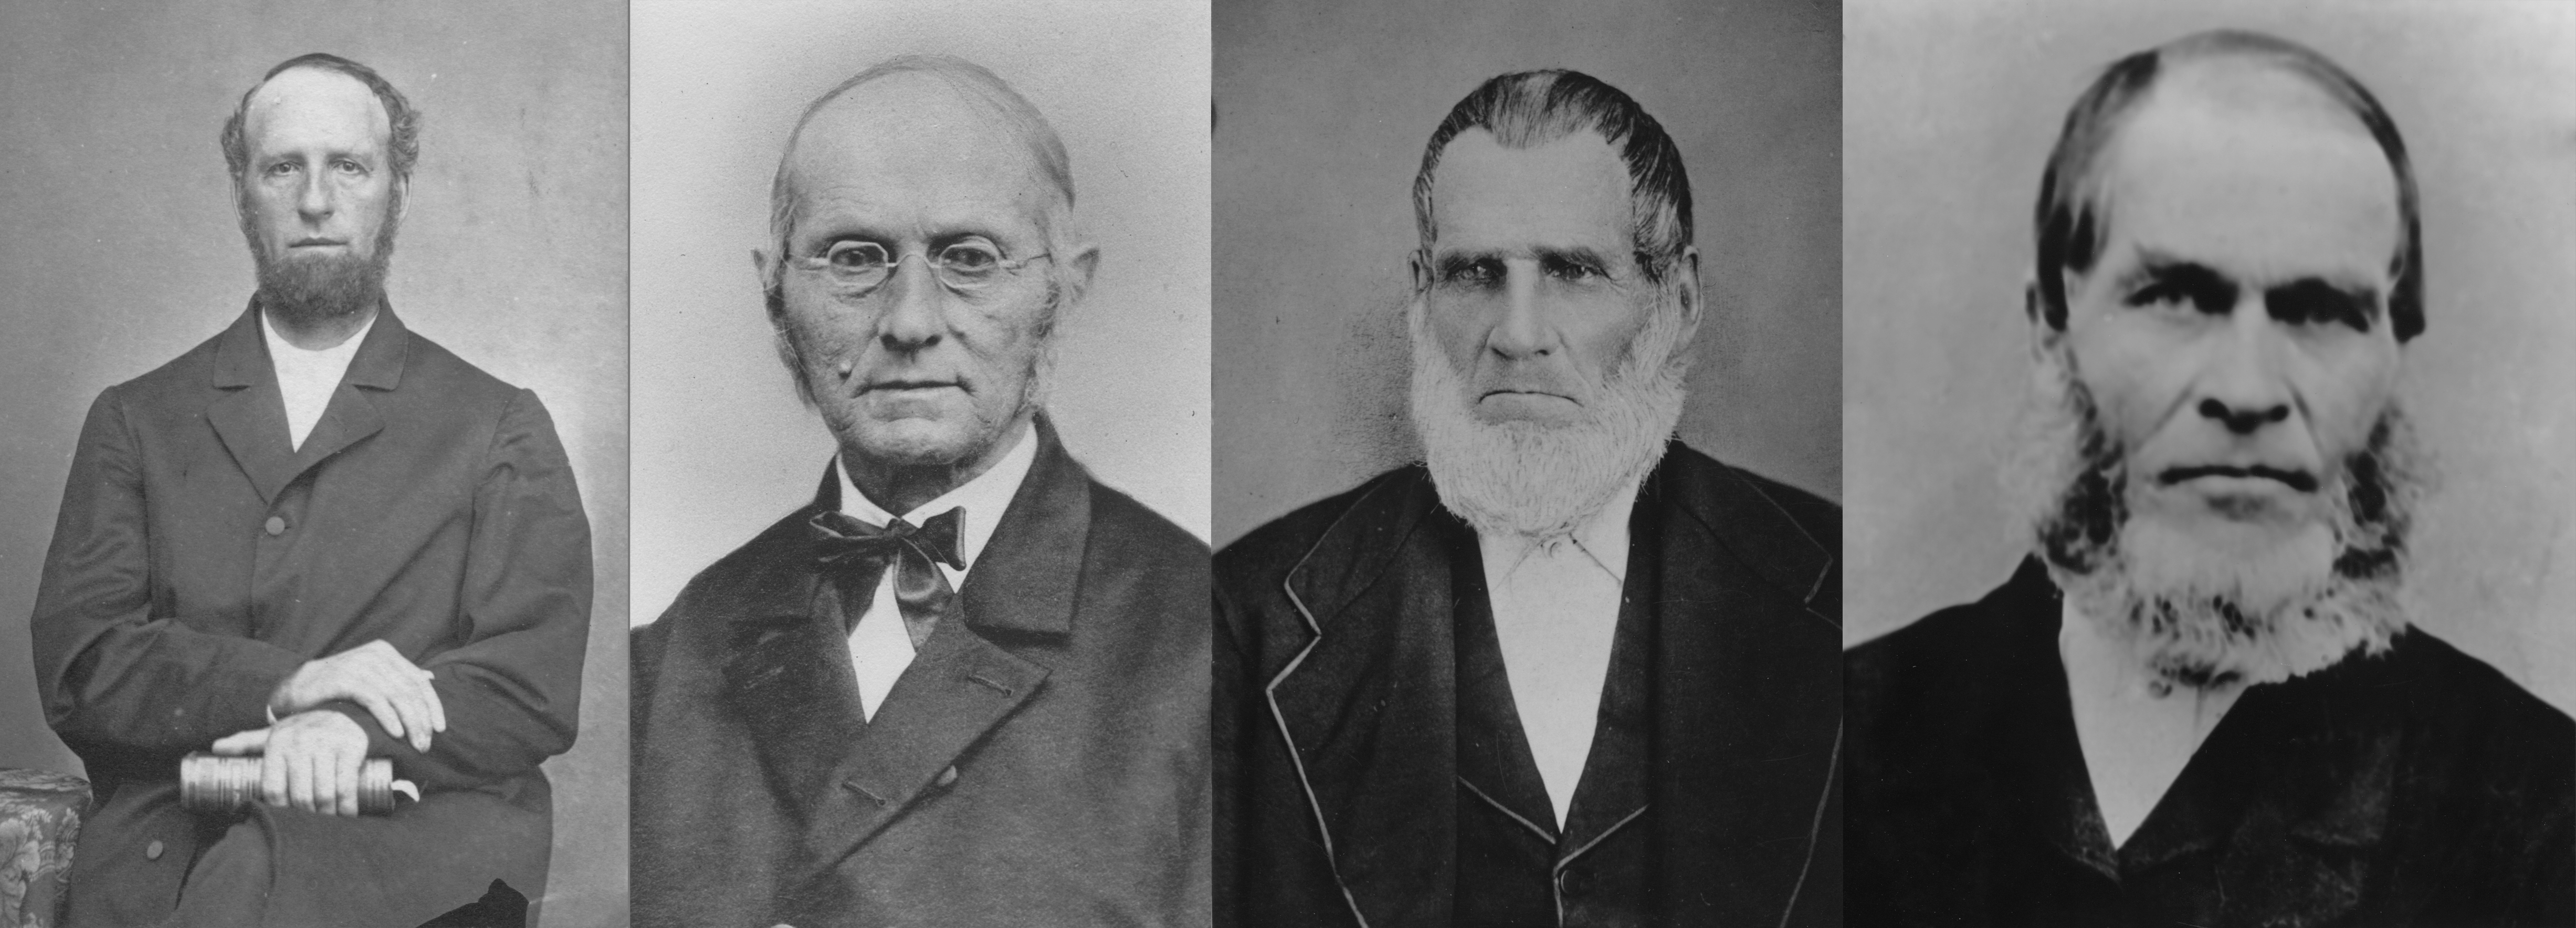
\includegraphics[width=1\linewidth]{images/james-white-joseph-bates-stephen-pierce-hiram-edson.jpg}
    \caption*{James White, Joseph Bates, Stephen Pierce, Hiram Edson}
    \label{fig:pioneers}
\end{figure}

\egwnogap{Tijekom cijelog tog vremena nisam mogla razumjeti rezoniranje braće. Moj um je bio zaključan, kao da nisam mogla dokučiti značenje Pisma koje smo proučavali. To je bila jedna od najvećih tuga u mojem životu. \textbf{Bila sam u tom stanju uma dokle god se nisu sve \underline{točke principa naše vjere} razbistrile našim umovima u harmoniji sa Božjom Riječi}. Braća su znali da kada nisam u viziji, da ne mogu razumjeti ove stvari, i oni su prihvatili otkrivenja koja su mi dâna kao direktnu svjetlost s neba.}[SpTB02 57.1; 1904][https://egwwritings.org/read?panels=p417.291]

\egwnogap{Kroz dvije ili tri godine moj um je ostao zaključan za razumijevanje Pisma. U našemu radu, moj suprug i ja posjetili smo oca Andrews-a, koji je bio u velikim bolovima radi upalnog reumatizma. Molili smo se za njega. Položila sam svoju ruku na njegovu glavu, i rekla: ‘Oče Andrews, Gospodin Isus te iscjeljuje.’ Istog trenutka je bio iscjeljen. On je ustao i hodao po sobi, slaveći Boga, govoreći: ‘Nikada nisam to prije tako vidio. Anđeli Božji su u ovoj sobi.’ Božja slava se očitovala. Doimalo se da svjetlost sija kroz čitavu kuću, i anđeoska ruka je bila položena na moju glavu. Od tog vremena do sada bila sam sposobna razumjeti riječ Božju.}[SpTB02 57.2; 1904][https://egwwritings.org/read?panels=p417.292]

\egwnogap{\textbf{Koji bi to utjecaj mogao, u ovom dijelu povijesti, na nepošten, snažan način \underline{srušiti temelje naše vjere},—temelj koji je bio postavljen na početku našeg rada sa molitvom i proučavanjem Riječi i Otkrivenja? Na \underline{tom temelju} smo gradili \underline{posljednjih pedeset godina}. Smatraš li da nemam što reći kada vidim početak rada koji bi \underline{uklonio neke od stupova naše vjere}? Moram poslušati naredbu, ‘Suoči se!’}}[SpTB02 58.1; 1904][https://egwwritings.org/read?panels=p417.295]

\egwnogap{Imam najdublje osjećaje prema dr. Kelloggu. Dugi niz godina pokušavala sam ga čvrsto držati. Božja riječ mi je uvijek govorila: ‘Možeš mu pomoći.’ Ponekad se probudim u noći, hodam sobom i moleći se: ‘Gospodine, drži čvrsto dr. Kellogga. Nemoj ga pustiti. Drži ga postojanim. Pomaži njegove oči s nebeskim uljem, kako bi jasno sve vidio.’ Noć za noći, bila sam budna, proučavajući kako bih mu mogla pomoći. Gorljivo i često sam se molila da mu Gospodin ne dopusti da se odvrati od posvećujuće istine. Ovo je teret koji me tišti,—želja da se on sačuva od pogrešaka koji bi naštetili njegovoj duši i \textbf{ozlijedili sadašnju istinu}. Ali za neko vrijeme njegova su djela otkrila da ga upravlja neobičan duh. Gospod će ovo uzeti u svoje ruke. Moram nositi poruke upozorenja koje mi je Bog dao da nosim, a rezultate prepuštam Gospodinu. \textbf{Sada moram predstaviti tu stvar u njegovom pravom svjetlu; jer narod Božji ne smije biti zakinut}.}[SpTB02 58.2; 1904][https://egwwritings.org/read?panels=p417.296]

\egwnogap{\textbf{Mi smo Božji narod koji čuvamo Njegove zapovijedi. U posljednjih pedeset godina svaka faza hereze nam je bila nametnuta, kako bi zamračila naše umove glede naučavanja Riječi},\textbf{—posebice vezano za Kristovu službu u nebeskoj Svetinji, i poruke Neba za ove posljednje dane, koje su dane anđelima iz četrnaestog poglavlja Otkrivenja}. \textbf{Poruke svakog reda i vrste su bile nametnute Adventistima Sedmoga dana, da zauzmu mjesto istine, koja \underline{točkom za točkom} je bila tražena sa molitvom i proučavanjem, i potvrđena čudesnom silom Gospodnjom}. \textbf{Ali \underline{međaši} \underline{koji su nas učinili onime što jesmo}, \underline{biti će očuvani}, kao što je Bog naznačio kroz svoju riječ i svjedočanstvo Njegovog Duha}. \textbf{On nas poziva da se \underline{držimo čvrstim} zahvatom vjere, \underline{fundamentalnih principa} koji su \underline{zasnovani na neupitnom autoritetu}}.}[SpTB02 59.1; 1904][https://egwwritings.org/read?panels=p417.299]

Godine 1904, postojala je potreba upozoriti crkvu o nastojanju neprijatelja da iskorijeni temelj naše vjere. Postojala je potreba podsjetiti crkvu što sačinjava istinski temelj vjere Adventista Sedmog Dana. Izgleda kako su Adventisti u to vrijeme zaboravili \egwinline{kako nas je Gospodin vodio i Njegovo učenje u našoj prošlosti.}[LS 196.2; 1915][https://egwwritings.org/read?panels=p41.1083]

\egw{Koji bi to utjecaj mogao, u ovom dijelu povijesti, na nepošten, snažan način \textbf{srušiti temelje naše vjere},—temelj koji je bio postavljen \textbf{na početku našeg rada} sa molitvom i proučavanjem Riječi i Otkrivenja? Na \textbf{tom temelju} smo gradili \textbf{posljednjih pedeset godina}. Smatraš li da nemam što reći kada vidim početak rada koji bi \textbf{uklonio neke od stupova naše vjere}? Moram poslušati naredbu, ‘\textbf{Suoči se}!’}[SpTB02 58.1; 1904][https://egwwritings.org/read?panels=p417.295]

Što je to s čime se sestra White trebala suočiti?

\egwinline{U vremenu kada je objavljena knjiga ‘Živi Hram’} u noćnoj viziji su joj bili predstavljeni \egwinline{prikazi koji su ukazivali na približavanje neke opasnosti,} te da se za nju mora \egwinline{pripremiti pisanjem stvari koje joj je Bog objavio} \egwinline{\textbf{vezano za temeljne principe naše vjere}.}

Bila je \egwinline{upućena od strane Nebeskog glasnika da su neka rasuđivanja u knjizi ‘Živi Hram’ netočna i da će \textbf{ta razmišljanja odvesti u zabludu} umove onih koji nisu temeljito utemeljeni na \textbf{temeljnim principima} sadašnje istine.}

Dakle, što je bio zapravo problem s knjigom “Živi Hram”?

Ako ste skolar, ili adventistički povjesničar, ili teolog, ili samo student teologije, prije nego što date direktan odgovor da je problem bio panteizam, željeli bi smo vas ponovno uputiti na tekst. Sestra White je jasno ukazala na srž problema navodeći da rasuđivanja knjige “Živi Hram” \egwinline{uvode ono što je ništa više nego obična nagađanja vezano za \textbf{ličnost Boga i gdje je Njegova prisutnost}}.

Ne osporavamo problem panteizma u knjizi, ali bi smo vam željeli skrenuti pažnju sa Kelloggovih zabluda na svjetlost koju je Bog dao. Postoje dva načina kojim možemo pristupiti Kelloggovoj krizi. Jedan način je adresirati panteizam, a drugi je adresirati \egwinline{\textbf{ličnost Boga} i \textbf{gdje je Njegova prisutnost}}. Jedan način je istraživati zabludu, a drugi način je istraživati Istinu. Jedan način je seciranje tame, dok drugi način je okrepljivanje sa izvora Istine. Mi smo odabrali ovaj drugi način, te je to jedan od razloga zašto ova knjiga je različita od stotinu drugih napisanih na temu Kelloggove krize. Tema ove knjige nije panteizam, niti bilo koja druga zabluda, već Istina, ono što je Bog objavio glede Svoje \emcap{ličnosti} i Njegove prisutnosti. To je bio stvarni problem Kelloggove knjige.

Smatramo da postoji velika opasnost u seciranju tame i zablude jer nas to lagano može odvesti u zabludu. Problem sa zabludom je taj što sami možemo biti zavedeni ne znajući da smo zavedeni! Čvrsto vjerujemo da je Ellen White bila Božji prorok i da je primala svjetlost od Boga koji je \bible{svjetlost i tame u njemu nema nikakve}[1 Ivanova 1:5]. Iz tog razloga ne očekujemo od sestre White da nam objasni zabludu u knjizi “Živi Hram”. Mnogi su joj prilazili sa zahtjevom da \egwinline{objasni stajališta u knjizi ‘Živi Hram’}. Odgovorila je \egwinline{Oni su neobjašnjivi}. Njezin cilj nije bio seciranje zablude već donijeti svjetlo o Istini o \emcap{ličnosti Boga} i Njegovoj prisutnosti. Iz tog razloga je skretala pažnju ljudi na iskustvo i istine kojima je Bog utemeljio crkvu Adventista Sedmoga Dana. Te istine su nam dane u našim ranim danima. Ukoliko našu pažnju smetnemo sa \emcap{ličnosti Boga} i počnemo se baviti panteizmom, izgubiti ćemo priliku prisjetiti se \egwinline{\textbf{kako nas je Gospodin vodio}, i \textbf{Njegovo učenje} u našoj \textbf{prošlosti}}. U tom svjetlu želimo izraziti zabrinutost za pristup Kelloggovoj krizi kroz panteističku prizmu, jer \egwinline{staza istine leži blizu staze zablude, i obje staze mogu izgledati jednake}; rješenje je da budemo \egwinline{temeljito utemeljeni na \textbf{temeljnim principima} sadašnje istine}. Na drugom mjestu sestra White nas je upozorila na važnost ovih fundamentalnih principa.

\egw{Sotona nikako ne spava; on je posve budan i igra igru života za duše naroda Božjega. Doći će im s laskanjem svih vrsta, u nadi da će ih navesti da odstupe od svoje odanosti. \textbf{Želi im skrenuti pozornost sa stvarnih problema na lažne teorije}.}[Ms132-1903.42; 1904][https://egwwritings.org/read?panels=p9056.56]

Zato posvetimo našu pažnju stvarnim problemima umjesto lažnim teorijama.

% Temelj Naše Vjere

\begin{titledpoem}
    \stanza{
        Istine stup, čvrsto stoji, \\
        Kroz oluje sve opstoji. \\
        Temelj vjere, Božji dar, \\
        Što ga gradi nebeski Zidar.
    }

    \stanza{
        Čuvaj se onih koji žele, \\
        Da temelje naše dijele. \\
        Identitet naš u njima jest, \\
        Božja objava, vječna čest.
    }

    \stanza{
        Na platformi čvrstoj stoj, \\
        Gdje svjetlost Božja vodi boj. \\
        Brani istinu svom snagom ti, \\
        Jer u njoj vječnost svijetli.
    }
\end{titledpoem}